%% Time-stamp: <2019-01-22 14:47:04 (marc)>
\documentclass[xcolor=x11names,compress,mathserif,handout]{beamer}

\usepackage{../includes/MarkMathCmds}


\newcommand{\hackspace}{\hspace{4.2mm}}
\newcommand{\showstudent}[1]{}



% talk/author information
\newcommand{\authorname}{Mark van der Wilk}
\newcommand{\authoremail}{m.vdwilk@imperial.ac.uk}
\newcommand{\authoraffiliation}{
 Department of Computing\\Imperial
  College London}
\newcommand{\authortwitter}{markvanderwilk}
\newcommand{\slidesettitle}{\imperialBlue{Building Probabilistic Models}}
\newcommand{\footertitle}{Building Probabilistic Models}
\newcommand{\location}{Imperial College London}
\newcommand{\talkDate}{{January 16, 2023}}

\usepackage{subfig}




\date{\imperialGray{\talkDate}}




% load defaults
\selectcolormodel{rgb}
\usepackage{ifxetex,ifluatex}
\newif\ifxetexorluatex
\ifxetex
  \xetexorluatextrue
\else
  \ifluatex
    \xetexorluatextrue
  \else
    \xetexorluatexfalse
  \fi
\fi

\usepackage{textpos}
%\usepackage{arabtex}
\usepackage{tikz}
\usetikzlibrary{decorations.markings}
\usetikzlibrary{arrows}
\usetikzlibrary{shapes}
\usetikzlibrary{plotmarks}
\usetikzlibrary{mindmap,trees,backgrounds}

\tikzstyle{every picture}+=[remember picture]

%\usepackage{movie15}
% \usepackage{pdfpages}
%\usepackage{xmpmulti}

\usepackage{anyfontsize}
\usepackage{wrapfig}
\usepackage{animate}
\usepackage{multirow}
\usepackage{multimedia}
\usepackage{xmpmulti}
%\usepackage[latin9]{inputenc}
\usepackage[english]{babel}
\usepackage{scalefnt}
\usepackage{verbatim}
\usepackage{url}
% \usepackage{pgf,pgfarrows,pgfnodes}
\usepackage{textpos}
\usepackage[tight,ugly]{units}
\usepackage{url}
\usepackage{bbm}
\usepackage[english]{babel}
\usepackage{fancyhdr}
\usepackage{bm} % correct bold symbols, like \bm
\usepackage{amsmath}
\usepackage{amsfonts}
\usepackage{amssymb}
\usepackage{mathrsfs}
\usepackage{mathtools}
\usepackage{color}
\usepackage{cancel}
\usepackage{algorithm}
\usepackage{algpseudocode}
\usepackage{mathrsfs}
\usepackage{listings}
\usepackage{graphicx} % for pdf, bitmapped graphics files
\usepackage{mathtools}
\usepackage{units}
\usepackage{subfig}
\usepackage{enumerate}
\usepackage{natbib}
\usepackage{dsfont}


\ifxetexorluatex
\usepackage{fontspec}
\setmainfont[Scale=0.8]{OpenDyslexic-Regular}
\else
\usefonttheme{professionalfonts}
\fi

\renewcommand{\vec}[1]{{\boldsymbol{{#1}}}} % vector
\newcommand{\mat}[1]{{\boldsymbol{{#1}}}} % matrix
% \newcommand{\KL}[2]{\mathrm{KL}(#1\|#2)} % KL divergence
\newcommand{\R}[0]{\mathds{R}} % real numbers
\newcommand{\Z}[0]{\mathds{Z}} % integers
\newcommand{\tr}[0]{\text{tr}} % trace
% \newcommand{\inv}{^{-1}}
% \DeclareMathOperator*{\diag}{diag}
\newcommand{\E}{\mathds{E}} % expectation
\newcommand{\var}{\mathds{V}}
\newcommand{\gauss}[2]{\mathcal{N}\big(#1,\,#2\big)}
\newcommand{\gaussx}[3]{\mathcal{N}\big(#1\,|\,#2,\,#3\big)}
\newcommand{\gaussBig}[2]{\mathcal{N}\left(#1,\,#2\right)}
\newcommand{\gaussxBig}[3]{\mathcal{N}\left(#1\,\left|\,#2,\,#3\right.\right)}
\newcommand{\Ber}[0]{\mathrm{Ber}} % Bernoulli distribution
\DeclareMathOperator{\cov}{Cov}
\ifxetexorluatex
\renewcommand{\T}[0]{^\top}
\renewcommand{\d}[0]{\text{d}} % derivative
\else
\newcommand{\T}[0]{^\top}
\renewcommand{\d}[0]{\text{d}} % derivative
\fi
% calculus
\newcommand{\pdiff}[1]{\frac{\partial}{\partial #1}}
\newcommand{\pdiffF}[2]{\frac{\partial #1}{\partial #2}}
\newcommand{\diffF}[2]{\frac{{\d}#1}{{\d}#2}}
\newcommand{\diffFII}[2]{\frac{{\d}^2 #1}{{\d}#2^2}}
\newcommand{\diff}[1]{\frac{{\d}}{{\d}#1}}
\newcommand{\diffII}[1]{\frac{{\d}^2}{{\d}#1^2}}
\newcommand{\class}[0]{\mathcal{C}}

\newcommand{\idx}[1]{^{(#1)}}
% \newcommand{\norm}[1]{\left\|#1\right\|}
\newcommand{\proj}[1]{\tilde{#1}}
\newcommand{\pcacoord}{z}
\newcommand{\pcacoordnew}{\zeta}
\newcommand{\latent}{z}
% \newcommand{\given}{\,|\,}
\newcommand{\genset}[1]{\mathrm{span}[#1]} % generating set
\newcommand{\set}[1]{\mathcal{#1}} % set
\newcommand{\fixgmfont}[1]{\scalebox{0.8}{#1}}



\usepackage{pifont}% http://ctan.org/pkg/pifont
\newcommand{\cmark}{{\color{green!40!black}\ding{51}}}%
\newcommand{\xmark}{{\color{red}\ding{55}}}%
\newcommand{\green}[1]{{\bf{\textcolor{green}{#1}}}}
\newcommand{\red}[1]{{\bf{\textcolor{red}{#1}}}}

\newcommand<>\red[1]{{\color#2[rgb]{1,0,0}#1}}
\newcommand<>\blue[1]{{\color#2[rgb]{0,0,1}#1}}
\newcommand<>\yellow[1]{{\color#2{camyellow}#1}}
\newcommand<>\green[1]{{\color#2[rgb]{0,0.6,0.0}#1}}
\newcommand<>\violet[1]{{\color#2[rgb]{0.6,0,0.6}#1}}
\newcommand<>\orange[1]{{\color#2[rgb]{1,0.5,0}#1}}
\newcommand<>\black[1]{{\color#2[rgb]{0,0,0}#1}}
\newcommand<>\steel[1]{{\color#2[rgb]{0,0,0.8}#1}}
\newcommand<>\darkblue[1]{{\color#2[rgb]{0,0,0.6}#1}}
\newcommand<>\lightblue[1]{{\color#2[rgb]{0.4,0.4,0.7}#1}}
\newcommand<>\gray[1]{{\color#2[rgb]{0.4,0.4,0.4}#1}}
\newcommand<>\greenish[1]{{\color#2[rgb]{0.45, 0.66, 0.45}#1}}
\newcommand<>\redish[1]{{\color#2[rgb]{0.7843    0.3706    0.3706}#1}}
\definecolor{redishTIKZ}{rgb}{0.7843, 0.3706, 0.3706}
\definecolor{imperialBlue}{rgb}{0.058, 0.219, 0.418}
\definecolor{aimsbrown}{rgb}{0.539, 0.117, 0.015}
% \definecolor{imperialGray}{rgb}{0.414, 0.488, 0.671 }
\definecolor{imperialGray}{RGB}{109,153, 204}
\definecolor{aimslightbrown}{RGB}{138,88,84}
\newcommand<>\imperialBlue[1]{{\color#2[rgb]{0.058, 0.219, 0.418}#1}}
\newcommand<>\aimsbrown[1]{{\color#2[rgb]{0.539, 0.117, 0.015}#1}}
%\newcommand<>\imperialGray[1]{{\color#2[rgb]{0.414, 0.488, 0.671}#1}}
\newcommand<>\imperialGray[1]{{\color#2[RGB]{109,153, 204}#1}}
\newcommand<>\aimslightbrown[1]{{\color#2[RGB]{138,88,84}#1}}
\newcommand<>\lightgray[1]{{\color#2[rgb]{0.8,0.8,0.8}#1}}
%\newcommand<>\highlightcolor[1]{{\color#2[rgb]{0,0,1}#1}}
\newcommand{\highlight}[1]{{\bf\steel{#1}}}
%\newcommand{\newblock}[0]{}

%\newcommand{\arrow}[0]{\includegraphics[height=5pt]{./figures/arrow}\hspace{3pt}}

\renewcommand{\emph}[1]{\textbf{\steel{{#1}}}}

\renewcommand{\alert}[1]{{\bf\red{{#1}}}}

\newcommand{\arrow}{
\begin{tikzpicture}
\draw [black!40!green, fill=black!40!green] (0,-0.12) -- (0,0.12) --
(0.15,0);
\draw [black!40!green, fill=black!40!green] (0.15,-0.12) -- (0.15,0.12) --
(0.3,0); 
\end{tikzpicture}
}

\geometry{left=0.45cm,top=0cm,right=0.45cm}


\newcommand{\logoimagepath}{./figures/imperial}
\newcommand{\highlightcolor}{blue!80!black}
%\newcommand{\headbarcolor}{imperialBlue}
\newcommand{\headbarcolor}{imperialBlue}
\institute{}

\newcommand{\coursetitle}{}

\newcommand{\slidesetsubtitle}{}
\newcommand{\slidesetnumber}{01}
\usefonttheme{professionalfonts}


\usetikzlibrary{decorations.fractals}
% tikzlibrary.code.tex
%
% Copyright 2010-2011 by Laura Dietz
% Copyright 2012 by Jaakko Luttinen
%
% The MIT License
%
% See LICENSE file for more details.

% Load other libraries
\usetikzlibrary{shapes}
\usetikzlibrary{fit}
\usetikzlibrary{chains}
\usetikzlibrary{arrows}

% Latent node
\tikzstyle{latent} = [circle,fill=white,draw=black,inner sep=1pt,
minimum size=20pt, font=\fontsize{10}{10}\selectfont, node distance=1]
% Observed node
\tikzstyle{obs} = [latent,fill=gray!25]
% Constant node
\tikzstyle{const} = [rectangle, inner sep=0pt, node distance=1]
% Factor node
\tikzstyle{factor} = [rectangle, fill=black,minimum size=5pt, inner
sep=0pt, node distance=0.4]
% Deterministic node
\tikzstyle{det} = [latent, diamond]

% Plate node
\tikzstyle{plate} = [draw, rectangle, rounded corners, fit=#1]
% Invisible wrapper node
\tikzstyle{wrap} = [inner sep=0pt, fit=#1]
% Gate
\tikzstyle{gate} = [draw, rectangle, dashed, fit=#1]

% Caption node
\tikzstyle{caption} = [font=\footnotesize, node distance=0] %
\tikzstyle{plate caption} = [caption, node distance=0, inner sep=0pt,
below left=5pt and 0pt of #1.south east] %
\tikzstyle{factor caption} = [caption] %
\tikzstyle{every label} += [caption] %

%\pgfdeclarelayer{b}
%\pgfdeclarelayer{f}
%\pgfsetlayers{b,main,f}

% \factoredge [options] {inputs} {factors} {outputs}
\newcommand{\factoredge}[4][]{ %
  % Connect all nodes #2 to all nodes #4 via all factors #3.
  \foreach \f in {#3} { %
    \foreach \x in {#2} { %
      \path (\x) edge[-,#1] (\f) ; %
      %\draw[-,#1] (\x) edge[-] (\f) ; %
    } ;
    \foreach \y in {#4} { %
      \path (\f) edge[->, >={triangle 45}, #1] (\y) ; %
      %\draw[->,#1] (\f) -- (\y) ; %
    } ;
  } ;
}

% \edge [options] {inputs} {outputs}
\newcommand{\edge}[3][]{ %
  % Connect all nodes #2 to all nodes #3.
  \foreach \x in {#2} { %
    \foreach \y in {#3} { %
      \path (\x) edge [->, >={triangle 45}, #1] (\y) ;%
      %\draw[->,#1] (\x) -- (\y) ;%
    } ;
  } ;
}

% \factor [options] {name} {caption} {inputs} {outputs}
\newcommand{\factor}[5][]{ %
  % Draw the factor node. Use alias to allow empty names.
  \node[factor, label={[name=#2-caption]#3}, name=#2, #1,
  alias=#2-alias] {} ; %
  % Connect all inputs to outputs via this factor
  \factoredge {#4} {#2-alias} {#5} ; %
}

% \plate [options] {name} {fitlist} {caption}
\newcommand{\plate}[4][]{ %
  \node[wrap=#3] (#2-wrap) {}; %
  \node[plate caption=#2-wrap] (#2-caption) {#4}; %
  \node[plate=(#2-wrap)(#2-caption), #1] (#2) {}; %
}

% \gate [options] {name} {fitlist} {inputs}
\newcommand{\gate}[4][]{ %
  \node[gate=#3, name=#2, #1, alias=#2-alias] {}; %
  \foreach \x in {#4} { %
    \draw [-*,thick] (\x) -- (#2-alias); %
  } ;%
}

% \vgate {name} {fitlist-left} {caption-left} {fitlist-right}
% {caption-right} {inputs}
\newcommand{\vgate}[6]{ %
  % Wrap the left and right parts
  \node[wrap=#2] (#1-left) {}; %
  \node[wrap=#4] (#1-right) {}; %
  % Draw the gate
  \node[gate=(#1-left)(#1-right)] (#1) {}; %
  % Add captions
  \node[caption, below left=of #1.north ] (#1-left-caption)
  {#3}; %
  \node[caption, below right=of #1.north ] (#1-right-caption)
  {#5}; %
  % Draw middle separation
  \draw [-, dashed] (#1.north) -- (#1.south); %
  % Draw inputs
  \foreach \x in {#6} { %
    \draw [-*,thick] (\x) -- (#1); %
  } ;%
}

% \hgate {name} {fitlist-top} {caption-top} {fitlist-bottom}
% {caption-bottom} {inputs}
\newcommand{\hgate}[6]{ %
  % Wrap the left and right parts
  \node[wrap=#2] (#1-top) {}; %
  \node[wrap=#4] (#1-bottom) {}; %
  % Draw the gate
  \node[gate=(#1-top)(#1-bottom)] (#1) {}; %
  % Add captions
  \node[caption, above right=of #1.west ] (#1-top-caption)
  {#3}; %
  \node[caption, below right=of #1.west ] (#1-bottom-caption)
  {#5}; %
  % Draw middle separation
  \draw [-, dashed] (#1.west) -- (#1.east); %
  % Draw inputs
  \foreach \x in {#6} { %
    \draw [-*,thick] (\x) -- (#1); %
  } ;%
}


% Copyright (C) 2016  Joseph Rabinoff

% ipe2tikz is free software; you can redistribute it and/or modify it under
% the terms of the GNU General Public License as published by the Free
% Software Foundation; either version 3 of the License, or (at your option)
% any later version.

% ipe2tikz is distributed in the hope that it will be useful, but WITHOUT ANY
% WARRANTY; without even the implied warranty of MERCHANTABILITY or FITNESS
% FOR A PARTICULAR PURPOSE.  See the GNU General Public License for more
% details.

% You should have received a copy of the GNU General Public License along with
% ipe2tikz; if not, you can find it at "http://www.gnu.org/copyleft/gpl.html",
% or write to the Free Software Foundation, Inc., 675 Mass Ave, Cambridge, MA
% 02139, USA.


% ipe compatibility TikZ styles

\usetikzlibrary{arrows.meta}

\makeatletter

% These should behave almost exactly like ipe arrows.  They disable correcting
% for the miter length and line width.  This is important for visual consistency
% with ipe, since ipe arrows get much larger when the line width is increased.
% They also use the line join and cap styles from the main path.  These are very
% simple arrows: there is no harpoon version, and the convex hull computation is
% sloppy.

\pgfdeclarearrow{
  name = ipe _linear,
  defaults = {
    length = +1bp,
    width  = +.666bp,
    line width = +0pt 1,
  },
  setup code = {
    % Control points
    \pgfarrowssetbackend{0pt}
    \pgfarrowssetvisualbackend{
      \pgfarrowlength\advance\pgf@x by-.5\pgfarrowlinewidth}
    \pgfarrowssetlineend{\pgfarrowlength}
    \ifpgfarrowreversed
      \pgfarrowssetlineend{\pgfarrowlength\advance\pgf@x by-.5\pgfarrowlinewidth}
    \fi
    \pgfarrowssettipend{\pgfarrowlength}
    % Convex hull
    \pgfarrowshullpoint{\pgfarrowlength}{0pt}
    \pgfarrowsupperhullpoint{0pt}{.5\pgfarrowwidth}
    % The following are needed in the code:
    \pgfarrowssavethe\pgfarrowlinewidth
    \pgfarrowssavethe\pgfarrowlength
    \pgfarrowssavethe\pgfarrowwidth
  },
  drawing code = {
    \pgfsetdash{}{+0pt}
    \ifdim\pgfarrowlinewidth=\pgflinewidth\else\pgfsetlinewidth{+\pgfarrowlinewidth}\fi
    \pgfpathmoveto{\pgfqpoint{0pt}{.5\pgfarrowwidth}}
    \pgfpathlineto{\pgfqpoint{\pgfarrowlength}{0pt}}
    \pgfpathlineto{\pgfqpoint{0pt}{-.5\pgfarrowwidth}}
    \pgfusepathqstroke
  },
  parameters = {
    \the\pgfarrowlinewidth,%
    \the\pgfarrowlength,%
    \the\pgfarrowwidth,%
  },
}


\pgfdeclarearrow{
  name = ipe _pointed,
  defaults = {
    length = +1bp,
    width  = +.666bp,
    inset  = +.2bp,
    line width = +0pt 1,
  },
  setup code = {
    % Control points
    \pgfarrowssetbackend{0pt}
    \pgfarrowssetvisualbackend{\pgfarrowinset}
    \pgfarrowssetlineend{\pgfarrowinset}
    \ifpgfarrowreversed
      \pgfarrowssetlineend{\pgfarrowlength}
    \fi
    \pgfarrowssettipend{\pgfarrowlength}
    % Convex hull
    \pgfarrowshullpoint{\pgfarrowlength}{0pt}
    \pgfarrowsupperhullpoint{0pt}{.5\pgfarrowwidth}
    \pgfarrowshullpoint{\pgfarrowinset}{0pt}
    % The following are needed in the code:
    \pgfarrowssavethe\pgfarrowinset
    \pgfarrowssavethe\pgfarrowlinewidth
    \pgfarrowssavethe\pgfarrowlength
    \pgfarrowssavethe\pgfarrowwidth
  },
  drawing code = {
    \pgfsetdash{}{+0pt}
    \ifdim\pgfarrowlinewidth=\pgflinewidth\else\pgfsetlinewidth{+\pgfarrowlinewidth}\fi
    \pgfpathmoveto{\pgfqpoint{\pgfarrowlength}{0pt}}
    \pgfpathlineto{\pgfqpoint{0pt}{.5\pgfarrowwidth}}
    \pgfpathlineto{\pgfqpoint{\pgfarrowinset}{0pt}}
    \pgfpathlineto{\pgfqpoint{0pt}{-.5\pgfarrowwidth}}
    \pgfpathclose
    \ifpgfarrowopen
      \pgfusepathqstroke
    \else
      \ifdim\pgfarrowlinewidth>0pt\pgfusepathqfillstroke\else\pgfusepathqfill\fi
    \fi
  },
  parameters = {
    \the\pgfarrowlinewidth,%
    \the\pgfarrowlength,%
    \the\pgfarrowwidth,%
    \the\pgfarrowinset,%
    \ifpgfarrowopen o\fi%
  },
}


% For correcting minipage width in stretched nodes
\newdimen\ipeminipagewidth
\def\ipestretchwidth#1{%
  \pgfmathsetlength{\ipeminipagewidth}{#1/\ipenodestretch}}

\tikzstyle{ipe import} = [
  % General ipe defaults
  x=1bp, y=1bp,
%
  % Nodes
  ipe node stretch/.store in=\ipenodestretch,
  ipe stretch normal/.style={ipe node stretch=1},
  ipe stretch normal,
  ipe node/.style={
    anchor=base west, inner sep=0, outer sep=0, scale=\ipenodestretch
  },
%
  % Use a special key for the mark scale, so that the default can be overriden.
  % (This doesn't happen with the scale= key; those accumulate.)
  ipe mark scale/.store in=\ipemarkscale,
%
  ipe mark tiny/.style={ipe mark scale=1.1},
  ipe mark small/.style={ipe mark scale=2},
  ipe mark normal/.style={ipe mark scale=3},
  ipe mark large/.style={ipe mark scale=5},
%
  ipe mark normal, % Set default
%
  ipe circle/.pic={
    \draw[line width=0.2*\ipemarkscale]
      (0,0) circle[radius=0.5*\ipemarkscale];
    \coordinate () at (0,0);
  },
  ipe disk/.pic={
    \fill (0,0) circle[radius=0.6*\ipemarkscale];
    \coordinate () at (0,0);
  },
  ipe fdisk/.pic={
    \filldraw[line width=0.2*\ipemarkscale]
      (0,0) circle[radius=0.5*\ipemarkscale];
    \coordinate () at (0,0);
  },
  ipe box/.pic={
    \draw[line width=0.2*\ipemarkscale, line join=miter]
      (-.5*\ipemarkscale,-.5*\ipemarkscale) rectangle
      ( .5*\ipemarkscale, .5*\ipemarkscale);
    \coordinate () at (0,0);
  },
  ipe square/.pic={
    \fill
      (-.6*\ipemarkscale,-.6*\ipemarkscale) rectangle
      ( .6*\ipemarkscale, .6*\ipemarkscale);
    \coordinate () at (0,0);
  },
  ipe fsquare/.pic={
    \filldraw[line width=0.2*\ipemarkscale, line join=miter]
      (-.5*\ipemarkscale,-.5*\ipemarkscale) rectangle
      ( .5*\ipemarkscale, .5*\ipemarkscale);
    \coordinate () at (0,0);
  },
  ipe cross/.pic={
    \draw[line width=0.2*\ipemarkscale, line cap=butt]
      (-.5*\ipemarkscale,-.5*\ipemarkscale) --
      ( .5*\ipemarkscale, .5*\ipemarkscale)
      (-.5*\ipemarkscale, .5*\ipemarkscale) --
      ( .5*\ipemarkscale,-.5*\ipemarkscale);
    \coordinate () at (0,0);
  },
%
  % Arrow sizes (for TikZ arrows)
  /pgf/arrow keys/.cd,
  ipe arrow normal/.style={scale=1},
  ipe arrow tiny/.style={scale=.4},
  ipe arrow small/.style={scale=.7},
  ipe arrow large/.style={scale=1.4},
  ipe arrow normal,
  /tikz/.cd,
%
  % Approximations to ipe arrows
  % Put in a style to allow to reset default scale when "ipe arrow normal" is
  % changed.  I think this is the only way, since all the parameters to arrows
  % are expanded when the tip is declared.
  ipe arrows/.style={
    ipe normal/.tip={
      ipe _pointed[length=1bp, width=.666bp, inset=0bp,
                   quick, ipe arrow normal]},
    ipe pointed/.tip={
      ipe _pointed[length=1bp, width=.666bp, inset=0.2bp,
                   quick, ipe arrow normal]},
    ipe linear/.tip={
      ipe _linear[length = 1bp, width=.666bp,
                  ipe arrow normal, quick]},
    ipe fnormal/.tip={ipe normal[fill=white]},
    ipe fpointed/.tip={ipe pointed[fill=white]},
    ipe double/.tip={ipe normal[] ipe normal},
    ipe fdouble/.tip={ipe fnormal[] ipe fnormal},
    % These should maybe use [bend], but that often looks bad unless it's on an
    % actual arc.
    ipe arc/.tip={ipe normal},
    ipe farc/.tip={ipe fnormal},
    ipe ptarc/.tip={ipe pointed},
    ipe fptarc/.tip={ipe fpointed},
  },
  ipe arrows, % Set default sizes
]

% I'm not sure how to do this in a .style, since the #args get confused.
\tikzset{
  rgb color/.code args={#1=#2}{%
    \definecolor{tempcolor-#1}{rgb}{#2}%
    \tikzset{#1=tempcolor-#1}%
  },
}

\makeatother

\endinput

\usetikzlibrary{matrix,positioning,decorations.pathreplacing}
\usetikzlibrary{calc,quotes,angles}
\usetikzlibrary{arrows, arrows.meta, patterns}

\usetikzlibrary{decorations.pathreplacing}
\tikzset{
    position label/.style={
       above = 3pt,
       text height = 2ex,
       text depth = 1ex
    }
}

% \usetikzlibrary{decorations.markings}
\tikzset{
  font={\fontsize{14pt}{12}\selectfont}
}



\useoutertheme[subsection=false,shadow]{miniframes}
\useinnertheme{default}
\usefonttheme{serif}
%\usepackage{palatino}
\usepackage{mathpazo}
%\usepackage{utopia}
\usepackage{stmaryrd} % for varodot, bigodot 
\usepackage{mathabx} % for \coAsterisk
%\usepackage{mnsymbol}
%\setbeamertemplate{itemize item}{\scriptsize\raise1.7pt\hbox{\donotcoloroutermaths$\Asterisk$}}
%\setbeamertemplate{itemize item}{\scriptsize\raise1.7pt\hbox{\donotcoloroutermaths$\varodot$}}
%\setbeamertemplate{itemize subitem}{\scriptsize\raise1.25pt\hbox{\donotcoloroutermaths$\rhd$}}

\usepackage{xifthen}% provides \isempty tesst

\setbeamerfont{title like}{shape=\scshape}
\setbeamerfont{frametitle}{}



\setbeamercolor*{lower separation line head}{bg=blue} 
\setbeamercolor*{normal text}{fg=black,bg=white} 
\setbeamercolor*{alerted text}{fg=red} 
\setbeamercolor*{example text}{fg=black} 
%\setbeamercolor*{frametitle}{fg=aimsbrown} 
\setbeamercolor*{frametitle}{fg=imperialBlue} 
\setbeamercolor*{structure}{fg=black} 
 
\setbeamercolor*{palette tertiary}{fg=black,bg=black!10} 
\setbeamercolor*{palette quaternary}{fg=black,bg=black!10} 

%\renewcommand{\(}{\begin{columns}}
%\renewcommand{\)}{\end{columns}}
%\newcommand{\<}[1]{\begin{column}{#1}}
%\renewcommand{\>}{\end{column}}

% ======================================
% custom commands 
\newcommand{\cemph}[1]{\textcolor{\highlightcolor}{#1}}
\newcommand{\calert}[1]{\textcolor{red}{#1}}

\setbeamertemplate{navigation symbols}{}
%\renewcommand\frametitle[1]{{\textsc{\Large \textcolor{\highlightcolor}{#1}}}\vspace{0.6cm}\par}

\setbeamertemplate{frametitle}
{
{\textsc\bf \insertframetitle}\vspace{0.2cm}\par
}


%%%%%%%%%%%%%%%%%%%%%%%%%%%%%%%%%%%%%%%%%%%%%%%%%%
\setbeamertemplate{headline}{% 
	\setbeamercolor{head1}{bg=\headbarcolor}
	 \hbox{%
  \begin{beamercolorbox}[wd=.01\paperwidth,ht=2.25ex,dp=50ex,center]{head1}%
  \fontsize{5}{5}\selectfont  
  \end{beamercolorbox}%
  }
  \vspace{-50ex}
}
\setbeamertemplate{footline}{
\begin{tiny}
\setbeamercolor{foot1}{fg=black,bg=gray!10}
\setbeamercolor{foot2}{fg=gray,bg=gray!15}
\setbeamercolor{foot3}{fg=gray,bg=gray!10}
\setbeamercolor{foot4}{fg=black,bg=gray!20}
\setbeamercolor{foot5}{fg=gray,bg=gray!15}
\setbeamercolor{foot6}{fg=black,bg=gray!20}

% taken from theme infolines and adapted
  \leavevmode%
  \hbox{%
  \begin{beamercolorbox}[wd=.45\paperwidth,ht=2.25ex,dp=1ex,center]{foot1}%
  \fontsize{5}{5}\selectfont
  \flushleft \hspace*{2ex}{\footertitle}
  \end{beamercolorbox}%
  % \begin{beamercolorbox}[wd=.08\paperwidth,ht=2.25ex,dp=1ex,center]{foot2}
  % \end{beamercolorbox}%
  %   \begin{beamercolorbox}[wd=.05\paperwidth,ht=2.25ex,dp=1ex,center]{foot3}
  % \end{beamercolorbox}%
    \begin{beamercolorbox}[wd=.45\paperwidth,ht=2.25ex,dp=1ex,center]{foot4}%
  \fontsize{5}{5}\selectfont
  \authorname\hspace{5mm}@\location, \talkDate%\ (\authorweb) 
  \end{beamercolorbox}%
  % \begin{beamercolorbox}[wd=.05\paperwidth,ht=2.25ex,dp=1ex,center]{foot5}
  % \end{beamercolorbox}%
  \begin{beamercolorbox}[wd=.1\paperwidth,ht=2.25ex,dp=1ex,right]{foot6}%
	\insertframenumber{}  \hspace*{2ex} 
  \end{beamercolorbox}}%
  \vskip0pt%
\end{tiny}
\vskip0pt
}


\setbeamercolor{block title}{bg=imperialBlue!45, fg=white}
\setbeamertemplate{blocks}[rounded][shadow=true]


\newenvironment<>{myblock}[1]{%
  \begin{actionenv}#2%
      \def\insertblocktitle{#1}%
      \par%
      \mode<presentation>{%
%       \setbeamercolor{block title}{fg=black,bg=aimslightbrown!50!white}
      \setbeamercolor{block title}{fg=black,bg=imperialBlue!45!white}
       \setbeamercolor{block body}{fg=black,bg=gray!20}
       \setbeamercolor{itemize item}{fg=blue!40!white}
       \setbeamertemplate{itemize item}[triangle]
     }%
      \usebeamertemplate{block begin}}
    {\par\usebeamertemplate{block end}\end{actionenv}}

\newenvironment<>{myblock2}[1]{%
  \begin{actionenv}#2%
      \def\insertblocktitle{#1}%
      \par%
      \mode<presentation>{%
       \setbeamercolor{block title}{fg=white,bg=blue!80!black}
       \setbeamercolor{block body}{fg=black,bg=gray!20}
       \setbeamercolor{itemize item}{fg=green!60!black}
       \setbeamertemplate{itemize item}[triangle]
     }%
      \usebeamertemplate{block begin}}
    {\par\usebeamertemplate{block end}\end{actionenv}}

\gdef\colchar#1#2{%
  \tikz[baseline]{%
%  \node[anchor=base,inner sep=2pt,outer sep=0pt,fill = #2!20]
%  {\large{#1}};
  \node[anchor=base,inner sep=1pt,outer sep=0pt,fill = #2!20]
  {{\fontsize{11}{13}\selectfont #1}};
    }%
}%
\gdef\drawfontframe#1#2{%
  \tikz[baseline]{%
  \node[anchor=base,inner sep=2pt,outer sep=0pt,fill = #2!20] {#1};
    }%
  }%


\makeatletter
\let\@@magyar@captionfix\relax
\makeatother

%%% Local Variables:
%%% mode: latex
%%% TeX-master: "2018-09-arusha-linear-regression"
%%% End:



\newif\iflattersubsect

\AtBeginSection[] {
    \begin{frame}<beamer>
    \frametitle{Overview} %
    \tableofcontents[currentsection]  
    \end{frame}
    \lattersubsectfalse
}

\AtBeginSubsection[] {
    \iflattersubsect
    \begin{frame}<Coming Next>
    \frametitle{Overview} %
    \tableofcontents[currentsubsection]  
    \end{frame}
    \fi
    \lattersubsecttrue
}

\begin{document}


%%%%%%%%%%%%%%%%%%%%%%%%%%%%%%%%%%%%%%%%%%%%%%%%%%%%%%

{\setbeamertemplate{footline}{}
\begin{frame}
\title{\slidesettitle}
%\subtitle{SUBTITLE}
\author{\footnotesize
  \textbf{\authorname}
 }

 %%% LOGO

% \begin{flushright}
%   % \begin{columns}
%   %   \column{0.5\hsize}
%   %   \column{0.45\hsize}
%
\includegraphics[height = 8mm]{./figures/qla}\hspace{2mm}
%     
\includegraphics[height = 8mm]{./figures/aims-rwanda}\\[2mm]
%
\includegraphics[height = 8mm]{./figures/imperial}
%%\end{columns}
%\end{flushright}

\vspace{-0cm}
%\begin{flushleft}
%\vspace{-1.5cm}{\small \textcolor{blue}{\coursetitle}}\\\vspace{2cm}
{\huge \slidesettitle \ifthenelse{\equal{\slidesetsubtitle}{}}%
    {}% if #1 is empty
    {: \\ {\large \slidesetsubtitle}}% if #1 is not empty
    } \\    
    %\vspace{20pt}
%\end{flushleft}
  
 
% this is all stuff below the talk title. make two columns, just in
% case you want to have a picture or a second affiliation here 
\begin{columns}[t]
\column{0.8\hsize}
%\begin{flushleft}
\begin{columns}[t]
\column{0.6\hsize}
\insertauthor \\[2mm]
\authoraffiliation\\[2mm]
\column{0.25\hsize}
\\[2mm]

\includegraphics[height = 0.3cm]{./figures/twitter}{\small @\authortwitter}\\[-1mm]
\mbox{\small \url{\authoremail}}
\end{columns}
\column{0.14\hsize}
\end{columns}
% \authorweb\\
\vspace{7mm}
% \aimslightbrown{The Nelson Mandela African Institute of Science and
%   Technology\\Arusha, Tanzania}\\[2mm]
\insertdate
%\end{flushleft}
\end{frame}
}

%%% Local Variables:
%%% mode: latex
%%% TeX-master: t
%%% End:

%%%%%%%%%%%%%%%%%%%%%%%%%%%%%%%%%%%%%%%%%%%%%%%%%%%%%%%%%%%




\begin{frame}{Questions}
  Last time, I gave examples of probabilistic reasoning, e.g.~colour preception:
  \begin{gather*}
    % P(C|L,\hyp_k) = \sum_i \colchar{$P(C|L,I=i)$}{green} P(I=i|\hyp_k)
    P(C|L,\hyp_k) = \sum_i \colchar{$P(C|L,I=i)$}{orange} \colchar{$P(I=i|\hyp_k)$}{orange} \\
    \colchar{$P(C|L,I=i)$}{orange} = \frac{P(L|C,I=i)P(C)}{P(L|I=i)}
  \end{gather*} \pause

\begin{itemize}
\item But why this structure? \pause
\item What assumptions were made? \pause
\item How should assumptions be expressed and communicated? \pause
\item How do we manipulate distributions to the form we want?\pause
\end{itemize}

\begin{center}
\Large How to systematically approach \\
a probabilistic modelling problem?
\end{center}
\end{frame}


\begin{frame}{Mathematical Modelling}
  Often, we can pose a mathematical model of a phenomenon:
  \begin{itemize}
  \item Reflection (Phong model, different symbol convention)
    \begin{center}
      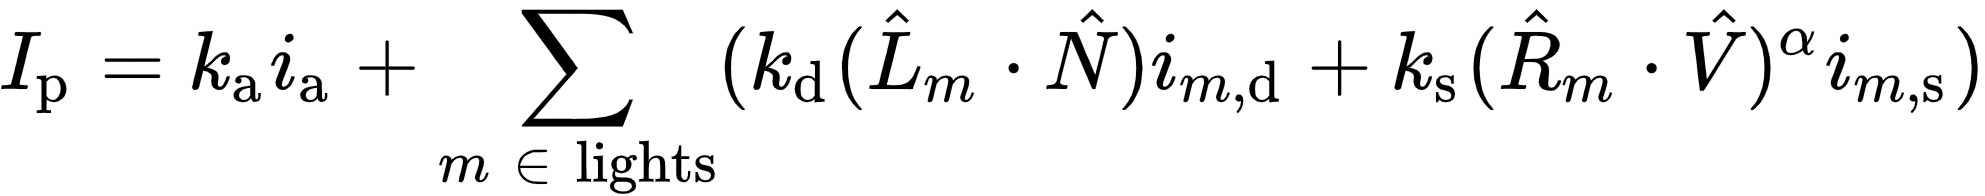
\includegraphics[width=0.8\textwidth]{./figures/phong-eqn.png}
    \end{center} \pause
  \item Movement of an object under gravity (Newton's laws)
    \begin{align}
      s_t &= \half \frac{m}{F} t^2 + v_0 t
    \end{align} \pause
  \end{itemize}

So if you are \emph{given} some quantities, you can make a prediction about another.
\end{frame}


\begin{frame}{From Mathematical Models to Probabilistic Models}
\begin{itemize}
\item A mathematical model expresses deterministic relationships. \pause
\item A probabilistic model expresses relationships with uncertainty. \pause
\item Often, probabilistic models are specified starting with a mathematical model. \pause
\item Mathematical relationships can help specify conditional distributions. \pause
\end{itemize}

\vspace{0.3cm}

Mathematical models are a \textit{special case} of deterministic models. Probability can still express certainty! \pause

E.g.~from Newton's laws:
\begin{align}
s_t &= \half \frac{m}{F} t^2 + v_0 t \\
p(s_t | v_0, m, F) &= \delta(s_t - \half \frac{m}{F} t^2 + v_0 t)
\end{align}

(Remember: $\int_{\mathcal R} \delta(\vx - \vy) \calcd\vx = 1$ if $\vy \in \mathcal R$, $0$ otherwise.)
\end{frame}



\begin{frame}{Probabilistic Models: Uncertain Quantities}
Given a mathematical model.
\begin{align}
p(s_t | v_0, m, F) &= \delta(s_t - \half \frac{m}{F} t^2 + v_0 t)
\end{align}

A certain relationship like this can be used to work back to uncertain quantities. \pause
Imagine we are uncertain about certain quantities:
\begin{align}
p(v_0, m, F) = \NormDist{v_0; \mu_v, 1.0}\delta(m - 1.0)\NormDist{F; \mu_F, 0.1}
\end{align} \pause

We can find how our uncertainty over the initial velocity $v_0$ changes by finding $p(v_0|s_t)$!
\end{frame}

\begin{frame}{Probabilistic Models: Uncertain Relationships}
\begin{itemize}
\item Is the relationship $p(s_t | v_0, m, F) = \delta(s_t - \half \frac{m}{F} t^2 + v_0 t)$ \emph{realistic}? \pause
\item If we did an initial value experiment, would we really measure \emph{exactly} the predicted value? \pause
\item Adding uncertainty makes predictions more \emph{realistic}, by allowing \emph{errors}.
\begin{align}
p(s_t | v_0, m, F) = \NormDist{s_t;  \half \frac{m}{F} t^2 + v_0 t, \sigma^2}
\end{align}
\end{itemize}
\end{frame}


\begin{frame}{Probability of Everything}
% What may be confusing about how we posed the dress problem, is that we immediately started
% from wanting to know what the posterior on the colour was. It is often difficult to write
% down the correct distributions for a posterior of interest directly.

% It's a good idea to start from a representation that 
How to make these intuitions \emph{systematic}? \pause \\

It's a good idea to start from a representation that:
\begin{enumerate}
\item clearly expresses the assumptions made in our model,
\item allows us to derive any distribution that we are interested in.
\end{enumerate}

\vspace{0.3cm} \pause

\begin{center}
{\large The joint distribution over all variables.} \\
{\Large The \emph{Probability of Everything}.}
\end{center}\pause

\vspace{-0.6cm}

\begin{gather}
p(x, y, z)
\end{gather} \pause
Any question we may want to answer corresponds to finding:
%\vspace{-0.4cm}
\begin{align}
p(x, z|y) = \frac{p(x, y, z)}{p(y)} && \text{or} && 
p(x | y) = \int \frac{p(x, y, z)}{p(y)} \calcd z
\end{align} \pause

\begin{itemize}
\item Observe a variable? Conditioning (i.e.~divide and renormalise).
\item Not interested in a variable? Marginalise.
\end{itemize}

\end{frame}


\begin{frame}{Building a Probabilistic Model: Statistical Approach}
Understanding how your variables causally interact gives you a factorisation of the joint.

% E.g.~changes in $X$ are caused only by Y and Z\pause

\pause

\begin{enumerate}
\item Identify all the variables that are relevant to your problem. \pause

\item Start with a variable that you will observe. \pause
% This is usually a good idea, since it depends on the variables that are hidden!

\item Determine which variables it depends on, and choose a sensible conditional distribution. \pause
\item Repeat previous step for one of the variables that you conditioned on.
\end{enumerate}
\end{frame}


\begin{frame}{Example: Lighting}
  \vspace{-1.0cm}
  \begin{columns}
    \hfill
    \centering
    \begin{column}{0.55\textwidth}
      \textbf{Step 1}: Identify all variables:
      \begin{itemize}
      \item Object colour $C$.
      \item Reflected light $L$.
      \item Illumination $I$.
      \end{itemize}
      Joint: $p(C, L, I)$.
    \end{column}
    \begin{column}{0.4\textwidth}  %%<--- here
          \begin{center}
            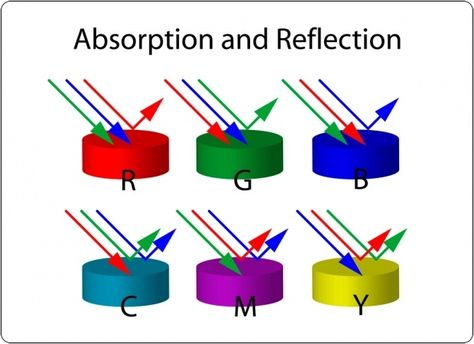
\includegraphics[width=\textwidth]{./figures/reflection.jpg}
          \end{center}
    \end{column}
    \hfill
  \end{columns} \pause


  \textbf{Step 2}: We observe the reflected light $L$. We have a model for the $L$ given $I$ and $C$: $p(L,C,I) = p(L|C,I)p(C, I)$. \pause

  \textbf{Step 3}: Let's pick $C$. Colour does not depend on illumination, so $p(C | I) = p(C)$, showing that $C$ and $I$ are independent.

\vspace{0.3cm} \pause
While we can use our knowledge for choosing $p(L|C, I)$, we need to choose subjective priors for $p(C)$ and $p(I)$.
\end{frame}

\begin{frame}{Finding the right posterior}
\begin{itemize}
\item Now that we have the joint, how do we find $p(C|L)$?
\item Remember: We need to find it in terms of the conditional distributions \emph{which we can actually evaluate}.
\item This is why starting with the joint is such a good idea! Given the definitions from the previous slide, we can evaluate it!
\end{itemize}
\begin{align}
p(C|L) &= \frac{\colchar{$p(C, L)$}{red}}{\colchar{$p(L)$}{red}} = \onslide<2->{\frac{\colchar{$\sum_I p(C, L, I)$}{orange}}{\colchar{$\sum_{C, I}p(C, L, I)$}{orange}}} \\
\onslide<3->{&= \frac{\sum_I \colchar{$p(L|C, I)$}{green} \colchar{$p(C)$}{green} \colchar{$p(I)$}{green}}{\dots}}
\end{align}

\onslide<4->{
We can take many different routes!
\begin{equation}
p(C|L) = \frac{\colchar{$p(L|C)$}{red}\colchar{$p(C)$}{green}}{p(L)} = \frac{\left[\sum_I \colchar{$p(L|C,I) p(I)$}{green}\right]\colchar{$p(C)$}{green}}{p(L)} % \colchar{$p(C|I, L)$}{red} \colchar{$p(I)$}{green} \,.
\end{equation}
Many roads lead to Rome, but starting from the joint \\
highlights assumptions
}
\end{frame}


\begin{frame}{Example: Burglars, Earthquakes, and Alarms}
\textit{``Fred lives in Los Angeles and commutes 60 miles to work. Whilst at work, he receives a phone-call from his neighbour saying that Fred’s burglar alarm is ringing. What is the probability that there was a burglar in his house today? While driving home to investigate, Fred hears on the radio that there was a small earthquake that day near his home. ‘Oh’, he says, feeling relieved, ‘it was probably the earthquake that set off the alarm’. What is the probability that there was a burglar in his house?''} \citep[][§21.1]{itila}
\vspace{0.2cm}

Q: How does the joint factorise? What conditionals should we define?
\vspace{-0.4cm}
\begin{itemize}[<+->]
\item Variables: \textbf{p}honecall, \textbf{a}larm, \textbf{b}urglar, \textbf{r}adio, \textbf{e}arthquake
\vspace{-0.2cm}
\begin{overprint}
\onslide*<1>{
\begin{flalign}
&p(p, a, b, r, e) = p(p, a, b, r, e)&
\end{flalign}
}
\onslide*<2>{
\begin{flalign}
&p(p, a, b, r, e) = p(p|a, b, r, e) p(a, b, r, e)&
\end{flalign}
}
\onslide*<3>{
\begin{flalign}
&p(p, a, b, r, e) = p(p|a) p(a, b, r, e)& % We assume you don't get a phonecall if there's an earthquake, or if the radio says something
\end{flalign}
}
\onslide*<4>{
\begin{flalign}
&p(p, a, b, r, e) = p(p|a) p(a | b, r, e) p(b, r, e)&
\end{flalign}
}
\onslide*<5>{
\begin{flalign}
&p(p, a, b, r, e) = p(p|a) p(a | b, e) p(b, r, e)&  % Alarm can go off due to earthquake or burglar
\end{flalign}
}
\onslide*<6>{
\begin{flalign}
&p(p, a, b, r, e) = p(p|a) p(a | b, e) p(b| r, e) p(r, e)&
\end{flalign}
}
\onslide*<7>{
\begin{flalign}
&p(p, a, b, r, e) = p(p|a) p(a | b, e) p(b) p(r, e)&
\end{flalign}
}
\onslide*<8->{
\begin{flalign}
&p(p, a, b, r, e) = p(p|a) p(a | b, e) p(b) p(r| e)p(e)&
\end{flalign}
}
\end{overprint}
\onslide<9->{
\vspace{-1.2cm}\item After selecting sensible conditionals, we have the joint.}
\end{itemize}
\end{frame}


\begin{frame}{Probabilistic Pipeline}
If your assumptions are good/correct, inference will give accurate results and good predictions.

  \begin{center}
    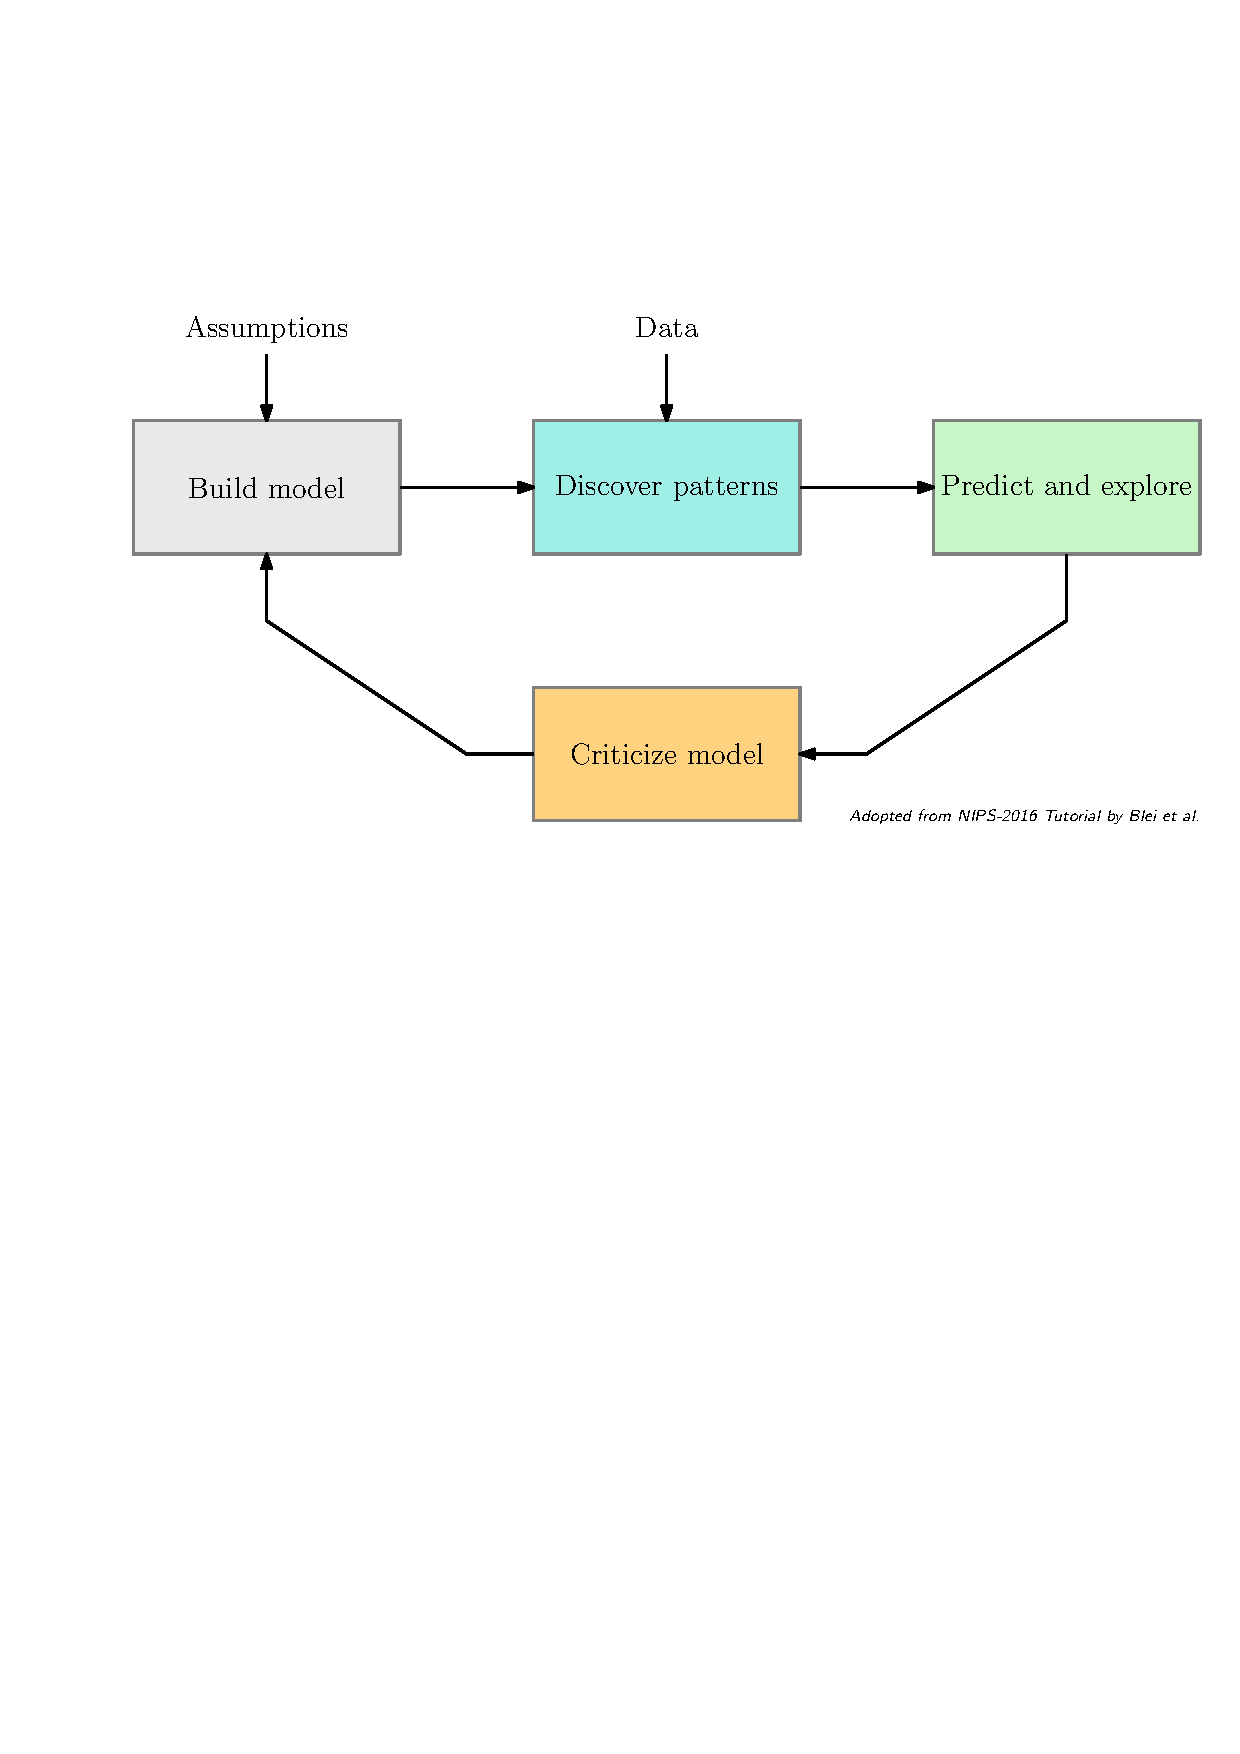
\includegraphics[width=0.58\hsize]{./figures/probabilistic_pipeline}
  \end{center}
  
  
  \begin{itemize}
  \item Good models \cemph{generate} data that is similar to the data we observe.
  \item \cemph{Predict and explore}: Sample from the prior, assess predictions.
  \item \emph{Criticize/revise the model}.
  \end{itemize}
\end{frame}



\begin{frame}{Building a Probabilistic Model: ML Approach}
Q: What happens if we don't have a mathematical/mechanistic model?
\begin{itemize}
\item For some problems, little is known about the process.
\item No known latent variables to use for creating a model.
\item We mainly want good prediction!
\end{itemize} \pause

\vspace{0.3cm}

All we really need is $p(\mathcal{D}_{\text{future}}, \mathcal{D}_{\text{observed}})$, so we can find the predictive distribution:
\begin{align}
p(\mathcal{D}_{\text{future}} | \mathcal{D}_{\text{observed}}) = \frac{p(\mathcal{D}_{\text{future}}, \mathcal{D}_{\text{observed}})}{p(\mathcal{D}_\text{observed})} \,.
\end{align}
\end{frame}


\begin{frame}{Latent Variables}
How do we create a joint with interesting relationships between the observed and future data? \pause
\begin{itemize}
\item Invent \emph{latent variables} that are \emph{common} to all data.
\begin{align}
p(\mathcal{D}_{\text{fut}}, \mathcal{D}_{\text{obs}}, \vz)
\end{align} \pause
\item For simplicity, often data is iid given latent variables.
\begin{align}
 p(\mathcal{D}_{\text{fut}}, \mathcal{D}_{\text{obs}}, \vz) = \prod_i p(\mathcal{D}_i|\vz) p(\vz)
\end{align} \pause
\item May not have a direct physical basis initially, but can turn out to be interpretable after training. \pause
\item Induces correlations between data, that can help to predict 
\begin{equation}
p(\mathcal{D}_\text{fut}, \mathcal{D}_{\text{obs}}) = \int p(\mathcal{D}_\text{fut}, \mathcal{D}_{\text{obs}}, \vz) \calcd{\vz}
\end{equation}
\end{itemize}
\end{frame}


\begin{frame}{Example: Linear Basis Function Regression}
Linear regression falls under this!
\begin{align}
p(\vy, \vy^*) &= \int \prod_i p(y_i|\vtheta) p(\vtheta) \calcd{\vtheta} \\
p(y_i|\vtheta) &= \NormDist{y_i; \vtheta\transpose\vphi(\vx), \sigma^2}
\end{align} \pause
\begin{itemize}
\item Do we really believe that the data we obtained was generated by sampling some parameters?
\item Do we really believe that the relationship is a sum of polynomials?
\item No, but it's useful for predicting!
\end{itemize} \pause
Similar, VAE (which we will also discuss).
\end{frame}


\begin{frame}{How do we know we have a good model?}
Model criticism is crucial!

Luckily, we have an objective metric on how well it's doing:
\pause
\begin{center}
\Large Predictive accuracy!
\end{center} \pause

\begin{itemize}
\item Hold-out test set.
\item Check where it is overconfident and underconfident.
\item Does it predict well when you change the setting?
\item Bayesian model selection (soon).
\end{itemize}

\vspace{0.3cm} \pause

The ML philosophy: if you predict well, you understand.
\end{frame}


\begin{frame}{Conclusion}
Summary:
\begin{itemize}
\item You can do anything with the joint.
\item Can create joints from understanding of the world.
\item Can create joints by just hypothesising relationships. \\ \pause Just make sure you validate your model...
\end{itemize} \pause

\vspace{0.3cm}

What you should be able to do:
\begin{itemize}
\item Create probabilistic model (i.e.~joints) by composing conditionals.
\item Apply sum and product rules to find desired posteriors.
\end{itemize}

\vspace{0.3cm} \pause

Reading \& exercises:
\begin{itemize}
\item Chapter 3 \citep{itila}.
\item Exercise: the burglar alarm \citep[][ch.21]{itila}
\item Exercise: bent coin \citep[][\S 3.2]{itila}
\item Exercise: legal evidence \citep[][\S 3.4]{itila}
\end{itemize}
\end{frame}















\begin{frame}[t,allowframebreaks]
\frametitle{References}
\linespread{1.0}
\tiny
% \bibliographystyle{abbrv}
\bibliographystyle{apalike}
\bibliography{../includes/pi-literature.bib}
\end{frame}















\end{document}
%%% Local Variables: 
%%% mode: latex
%%% TeX-master: t
%%% End: 
